\documentclass[12pt, a4paper, oneside]{ctexart}
\usepackage{amsmath, amsthm, amssymb, bm, color, framed, graphicx, hyperref, mathrsfs, float, caption,subfigure}
\usepackage[justification=centering]{caption}

% multi-column
\usepackage{tasks}
% itemize
\NewTasksEnvironment[label=(\arabic*), label-width=3ex]{exercise}
%\settasks{
% label = \theexercise.\arabic* ,
% item-indent = 2em ,
% label-width = 2em ,
% label-offset = 0pt
%}

\everymath{\displaystyle}

\title{\textbf{第六次随堂测试}}
\author{U08M11002 Fall 2023}
\date{2023 年 12 月 8 日}
\linespread{1}
\definecolor{shadecolor}{RGB}{241, 241, 255}

\newcounter{problemname}
\newenvironment{problem}{\stepcounter{problemname}\par\noindent\textbf{题目\arabic{problemname}. }}{\\\par}
\newenvironment{warning}{\begin{shaded}\par\noindent\textbf{提交作业方式:}}{\end{shaded}\par}

\begin{document}

\maketitle

\hspace{1em}

\pagestyle{plain}
  
\begin{problem}
    已知LTI系统 $H(s)$的零极图如下,已知 $h(0^+)=1$ \par
    \begin{figure}[h]
    \centering         %使图片居中放置
    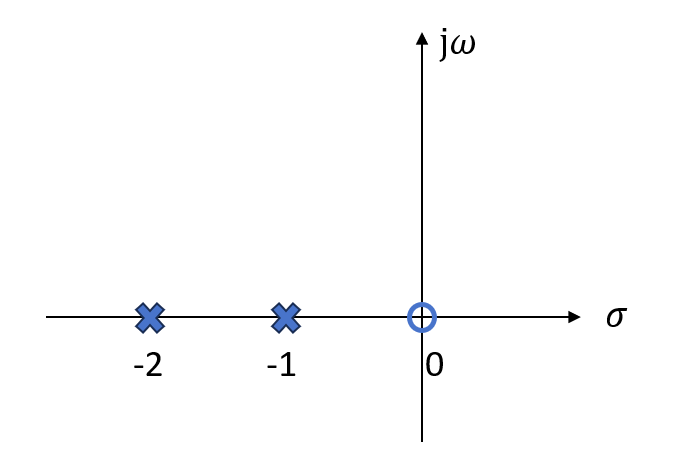
\includegraphics[scale=0.38]{TEST6.png}
    \end{figure}
    \begin{exercise}(1)
        \task 求 $H(s)$及$h(t)$。
        \task $f(t)=u(t)$时,求零状态响应$y_{zs}(t)$。
        \task 系统是否稳定?为什么?(只回答是/否不得分)
        \task 画出系统的模拟框图。
    \end{exercise}   
\quad
\end{problem}

\end{document}